
\begin{figure}[tb]
    \centering
    \begin{figure}[t]
    \centering
    \includegraphics[width=0.9\linewidth]{figures/png/block_diagram.png}
    \caption{Block diagram of the proposed model.}
    \label{fig:block diagram}
\end{figure}
    \caption{Control system overview and generalized coordinates.}
    \label{fig:controlsystem}
\end{figure}

This section details the control methods on the Mini Wheelbot, as visualized in~Fig.~\ref{fig:controlsystem}, that we later use in illustrative learning tasks in Sec.~\ref{sec:lbcexperiments}.
To this end, we first describe the system model (Sec.~\ref{sec:systemmodel}) and optimization-based identification of parameters from trajectory data (Sec.~\ref{sec:parameteridentification}), before introducing 
the state-feedback controller used for balancing (Sec.~\ref{sec:statefeedback}), and a nonlinear model-predictive controller for the orientation of the robot that is required for meaningful driving (Sec.~\ref{sec:nonlinearmpc}).
Finally, the stand-up in the roll and pitch direction and a half-flip are described (Sec.~\ref{sec:standup} and \ref{sec:flip}).
All implementations are available online\footnotemark[1].

We omit a detailed description on the estimation of the robots state, as we implement the existing method from~\cite{geist2022wheelbot} to fuse four gyroscope\footnote{Using corrected gyroscope measurement equations from the errata of~\cite{geist2022wheelbot}.}~$\omega_\text{B,i}$, four accelerometer~$a_\text{B,i}$, and two wheel encoder~$q_\text{D,R}$ measurements~(cf.~\cite{trimpe2010accelerometer,trimpe2012balancing,gajamohan2012cubli,muehlebach2016nonlinear} for details). Notably, the presented controllers are robust to alignment errors of the IMUs thus no calibration is needed.

\subsection{System Model}
\label{sec:systemmodel}
The Mini Wheelbot's state can be described as~$x~=~[\psi,\phi,\theta,\dot{\psi},\dot{\phi},\dot{\theta},q_\text{D}, q_\text{R}, \dot{q}_\text{D}, \dot{q}_\text{R}]^\top$.
The body orientation is expressed in Euler-like angles in yaw-roll-pitch order (see Fig.~\ref{fig:controlsystem}) with yaw~$\psi$ and roll~$\phi$ around the contact point coordinate system's~$\mathcal{C}_\text{z}$ axis and resulting~$\mathcal{C}^\prime_\text{x}$ axis, and pitch~$\theta$ around the drive motors axis of rotation that is aligned with~$\mathcal{D}_\text{y}$.
The angles of the wheels are~$q_\text{D,R}$ and the actions~$u~=~[\tau_\text{D}, \tau_\text{R}]^\top$ are the torques applied to driving~(bottom) and the reaction~(top) wheel.
The Mini Wheelbot's nonlinear, continuous-time dynamics of implicit form~$f_\text{ct}(x,\dot{x}, u, p)=0$ with parameters~$p$ can be derived using standard, multi-body methods~(e.g.,  Euler-Lagrange equations).
A detailed symbolic derivation using a computer algebra system is given in the supplementary code\footnotemark[1] and described in detail in~\cite{daud2017dynamic}.
The resulting differential equations have the form:
\begin{align}\label{eqn:eqnofmotion}
    \begin{split}M(\phi,\theta,p)&[\ddot{\phi},\ddot{\theta},\ddot{\psi}, \ddot{q}_\text{D}, \ddot{q}_\text{R}]^\top + b(\phi, \theta, \dot{\psi}, \dot{\phi}, \dot{\theta}, \dot{q}_\text{D}, \dot{q}_\text{R},p) \\ &+ g(\phi, \theta, \tau_\text{D}, \tau_\text{R},p)+\tau_{\psi}(\dot{\psi},p)= 0.
    \end{split}
\end{align}
The implicit dynamics~(\ref{eqn:eqnofmotion}) are parameterized by $p~=~[m_\text{D,R}, m_{B}, I_{\text{D}_\text{x,z}\text{,R}_\text{y,z}}, I_{\text{D}_\text{y}\text{,R}_\text{x}},
I_\text{B},
r_\text{D,R},
l_\text{D,R},
C_1, C_2]\in\mathbb{R}^{11}$, which consists of the masses and mass moments of inertia of the robot's body~$m_\text{B}$ and $I_\text{B}$ and reaction wheels~$m_\text{D,R}$ and ~$I_\text{D,R}$.
The mass moments of inertia are assumed to be diagonal and share values for multiple axis due to~(quasi-)symmetries.
Further, the radius of the wheels~$r_\text{D,R}$ and distance between rotation axis~$l_\text{D,R}$ enter as geometric parameters.
The rotational friction in the contact point is modeled as~$\tau_{\psi}=C_1\tanh(C_2\dot{\psi})$, where the constant~$C_1$ models the magnitude and~$C_2$ the slope of the friction.
The mass matrix~$M(\phi,\theta)$ is difficult to invert symbolically (i.e., symbolically computing~$\dot{x}=f_\text{expl}(x,u,p)$) and (\ref{eqn:eqnofmotion}) is stiff on a timescale relevant for controlling the yaw orientation.
Both issues motivate the use of implicit integrators~\cite{frey2023fast} for an accurate discrete-time model with time~$t\in\mathbb{N}$, that is:
\begin{align} \label{eqn:systemdynamics}
        x(t+1) = f_\text{dt}(x(t), u(t), p).
\end{align}


\subsection{Optimization-based Parameter Identification}
\label{sec:parameteridentification}
In this section, the optimization-based identification of the parameters~$p$ from data is described, which is similar to the methods presented in~\cite{bock1983recent,valluru2017development,simpson2023efficient,bodmer2024optimization}.
To this end, an optimization problem
\begin{align}
\begin{split}\label{eqn:sysid}
\min_{p\in\mathcal{P}, \hat{x},\hat{u}} & \sum_{i=0}^{N_\text{id}} \sum_{t=0}^{T_\text{id}}\|\hat{x}_i(t)-\bar{x}_i(t)\|^2_{Q_\text{id}}+\|\hat{u}_i(t)-\bar{u}_i(t)\|^2_{R_\text{id}}\\
\text{s.t.}\quad 
&\hat{u}_i(t)-\bar{u}_i(t)\in\mathcal{W},\;\forall t\in\mathbb{I}_{T_\text{id}},\forall i\in\mathbb{I}_{N_\text{id}}\\
&\hat{x}_i(t+1) = f_\text{dt}(\hat{x}(t), \hat{u}_i(t),p)
\;\forall t\in\mathbb{I}_{T_\text{id}},\forall i\in\mathbb{I}_{N_\text{id}}\\
\end{split}
\end{align}
is solved, where the parameters are constrained to reasonable box constraints~$\mathcal{P}$, the optimization objective consists of quadratic cost on the error between predicted~$\hat{x}$ and measured state~$\bar{x}$ and predicted~$\hat{u}$ and measured action~$\bar{u}$ over a finite horizon~$T_\text{id}$ and a set of trajectories~$N_\text{id}$.
The input disturbance constraint set~$\mathcal{W}$ can be conservatively approximated from direct measurements of the actuator torque ripple.
Quadratic cost matrices are chosen empirically as diagonal matrices~$Q_\text{id}=\text{diag}([100,1,1,10,10,10,0.1,0.1,0.1,0.1]^\top)$ and~$R_\text{id}=\text{diag}([100,100]^\top)$.

The optimization problem (\ref{eqn:sysid}) is implemented in CasADi~\cite{andersson2019casadi} and solved with IPOPT~\cite{wachter2006implementation}, which yields the optimal parameters~$p^*$.
A selection of trajectories from the dataset and the achieved prediction for the critical yaw state is plotted in Fig.~\ref{fig:sysid}.
In the following, the discrete-time dynamics~(\ref{eqn:systemdynamics}) with~$p^*$ substituted in will be referred to as~$f_\text{dt}(x(t), u(t))$, dropping the explicit dependency on~$p$ for ease of notation.

\begin{figure}[thpb]
    \centering
    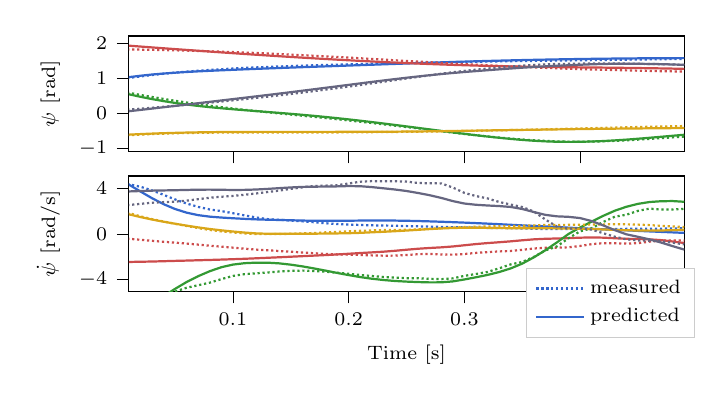
\begin{tikzpicture}[x=1in, y=1in]

    \definecolor{dimgrey85}{RGB}{85,85,85}
    \definecolor{gainsboro229}{RGB}{229,229,229}
    \definecolor{darkgray176}{RGB}{176,176,176}
    \definecolor{lightgray}{RGB}{211,211,211}
    \definecolor{lightgray204}{RGB}{204,204,204}

    \definecolor{color1}{rgb}{0.2, 0.4, 0.8}
    \definecolor{color2}{rgb}{0.8, 0.3, 0.3}
    \definecolor{color3}{rgb}{0.2, 0.6, 0.2}
    \definecolor{color4}{rgb}{0.85, 0.65, 0.1}
    \definecolor{color5}{rgb}{0.4, 0.4, 0.5}

    \begin{axis}[
    name=yaw,
    anchor=north west,
    width=3.4in,
    height=1.2in,
    legend cell align={left},
    legend style={
      fill opacity=1,
      draw opacity=1,
      text opacity=1,
      at={(1.02,-0.25)},
      anchor=south east,
      font=\scriptsize,
      draw=lightgray204
    },
    tick align=outside,
    tick pos=left,
    x grid style={darkgray176},
    xticklabels={},
    xmin=0.01, xmax=0.49,
    xtick style={color=black},
    y grid style={darkgray176},
    ylabel={$\psi$ [rad]},
    ytick style={color=black},
    tick label style={font=\scriptsize}, %
    label style={font=\scriptsize}, %
    ]
    \addplot [thick, color1, densely dotted]
    table {%
    0 0.963217
    0.01 1.00784
    0.02 1.0506
    0.03 1.09068
    0.04 1.12726
    0.05 1.15981
    0.06 1.18839
    0.07 1.21363
    0.08 1.23626
    0.09 1.25701
    0.1 1.27619
    0.11 1.29344
    0.12 1.30879
    0.13 1.32241
    0.14 1.33502
    0.15 1.34695
    0.16 1.35832
    0.17 1.36895
    0.18 1.37867
    0.19 1.38764
    0.2 1.39602
    0.21 1.40398
    0.22 1.4116
    0.23 1.41898
    0.24 1.42616
    0.25 1.43307
    0.26 1.43974
    0.27 1.44621
    0.28 1.45245
    0.29 1.45843
    0.3 1.46418
    0.31 1.46975
    0.32 1.47509
    0.33 1.4802
    0.34 1.48521
    0.35 1.49005
    0.36 1.49466
    0.37 1.49899
    0.38 1.50313
    0.39 1.50738
    0.4 1.51169
    0.41 1.51588
    0.42 1.51996
    0.43 1.52401
    0.44 1.52832
    0.45 1.5327
    0.46 1.53713
    0.47 1.54158
    0.48 1.54621
    0.49 1.55099
    };
    \addplot [thick, color1]
    table {%
    0 0.98407717719041
    0.01 1.03050770534316
    0.02 1.07096029652046
    0.03 1.10536591737476
    0.04 1.13412732437827
    0.05 1.15807216052356
    0.06 1.17824867528481
    0.07 1.1957221654346
    0.08 1.21145613146144
    0.09 1.2261681393311
    0.1 1.24019694212336
    0.11 1.25364048458015
    0.12 1.26659193135223
    0.13 1.27915554825876
    0.14 1.29148095158501
    0.15 1.30355491087084
    0.16 1.31537320434694
    0.17 1.32694357053663
    0.18 1.33837337491343
    0.19 1.3498117797264
    0.2 1.36131877092652
    0.21 1.37292543814125
    0.22 1.38462804589496
    0.23 1.3963766643955
    0.24 1.4080777727549
    0.25 1.41965190624679
    0.26 1.43102663047369
    0.27 1.44213711704192
    0.28 1.45293121485146
    0.29 1.46337619030868
    0.3 1.47343751537938
    0.31 1.48307568878493
    0.32 1.49226915964802
    0.33 1.50099148048949
    0.34 1.50920278466901
    0.35 1.51688495063845
    0.36 1.52406035867701
    0.37 1.53075030237738
    0.38 1.5369512147666
    0.39 1.54263295530941
    0.4 1.54778086332477
    0.41 1.55242981169564
    0.42 1.5566275581388
    0.43 1.56039046777279
    0.44 1.5636898660816
    0.45 1.56649448661359
    0.46 1.56882315388414
    0.47 1.57071077533546
    0.48 1.57216588685251
    0.49 1.57317957738902
    };
    \addplot [thick, color2, densely dotted]
    table {%
    0 1.82406
    0.01 1.82013
    0.02 1.81522
    0.03 1.80952
    0.04 1.80287
    0.05 1.79538
    0.06 1.78722
    0.07 1.77811
    0.08 1.76808
    0.09 1.7571
    0.1 1.74526
    0.11 1.73256
    0.12 1.71899
    0.13 1.70473
    0.14 1.68981
    0.15 1.67425
    0.16 1.65809
    0.17 1.64123
    0.18 1.62378
    0.19 1.60578
    0.2 1.58745
    0.21 1.5689
    0.22 1.55005
    0.23 1.53084
    0.24 1.51147
    0.25 1.49241
    0.26 1.47402
    0.27 1.45618
    0.28 1.4382
    0.29 1.41981
    0.3 1.40159
    0.31 1.38417
    0.32 1.36764
    0.33 1.35175
    0.34 1.33636
    0.35 1.3216
    0.36 1.30801
    0.37 1.29539
    0.38 1.28307
    0.39 1.27085
    0.4 1.25939
    0.41 1.24943
    0.42 1.24074
    0.43 1.23248
    0.44 1.22391
    0.45 1.21534
    0.46 1.20776
    0.47 1.20128
    0.48 1.19543
    0.49 1.18957
    };
    \addplot [thick, color2]
    table {%
    0 1.95281708820088
    0.01 1.92785220473126
    0.02 1.90304745137448
    0.03 1.8784360430858
    0.04 1.85406246456031
    0.05 1.82997565012477
    0.06 1.80616384060674
    0.07 1.7826278902627
    0.08 1.7593736500751
    0.09 1.73641194648207
    0.1 1.71377929229843
    0.11 1.69150113417816
    0.12 1.66962625274203
    0.13 1.64819845546346
    0.14 1.6272252876621
    0.15 1.60671858203118
    0.16 1.58669557262193
    0.17 1.56716390561003
    0.18 1.5481167969985
    0.19 1.52957892955046
    0.2 1.51162559178592
    0.21 1.49430465315353
    0.22 1.47758510864499
    0.23 1.46144645527528
    0.24 1.44600593816523
    0.25 1.43144190674035
    0.26 1.41780600181914
    0.27 1.40495281898006
    0.28 1.39268246048448
    0.29 1.38105640223272
    0.3 1.37036842911174
    0.31 1.3607687490585
    0.32 1.35214093196246
    0.33 1.34430152878319
    0.34 1.33721624731707
    0.35 1.33099479708174
    0.36 1.32569354310458
    0.37 1.32106101813475
    0.38 1.3167716085509
    0.39 1.31275955592751
    0.4 1.30911718045651
    0.41 1.30580916126018
    0.42 1.30251653762163
    0.43 1.29885347142249
    0.44 1.29464416115349
    0.45 1.29008721486974
    0.46 1.28534317907964
    0.47 1.28012680262669
    0.48 1.27395099787935
    0.49 1.26645510865579
    };
    \addplot [thick, color3, densely dotted]
    table {%
    0 0.646964
    0.01 0.584505
    0.02 0.524557
    0.03 0.466557
    0.04 0.41064
    0.05 0.357721
    0.06 0.308278
    0.07 0.261845
    0.08 0.217461
    0.09 0.175708
    0.1 0.137094
    0.11 0.100735
    0.12 0.0654328
    0.13 0.0308279
    0.14 -0.00292692
    0.15 -0.0359398
    0.16 -0.0684989
    0.17 -0.101153
    0.18 -0.134301
    0.19 -0.168234
    0.2 -0.203115
    0.21 -0.238976
    0.22 -0.27586
    0.23 -0.313613
    0.24 -0.352079
    0.25 -0.391052
    0.26 -0.430272
    0.27 -0.469783
    0.28 -0.509735
    0.29 -0.549562
    0.3 -0.587925
    0.31 -0.624199
    0.32 -0.658894
    0.33 -0.691151
    0.34 -0.719885
    0.35 -0.745905
    0.36 -0.768917
    0.37 -0.786347
    0.38 -0.799385
    0.39 -0.807334
    0.4 -0.807879
    0.41 -0.804495
    0.42 -0.797107
    0.43 -0.784012
    0.44 -0.768138
    0.45 -0.749769
    0.46 -0.72822
    0.47 -0.706403
    0.48 -0.685037
    0.49 -0.663217
    };
    \addplot [thick, color3]
    table {%
    0 0.6211499317257
    0.01 0.54337469299529
    0.02 0.471815631988583
    0.03 0.40665407378849
    0.04 0.348124302595699
    0.05 0.296217941142951
    0.06 0.250619710197404
    0.07 0.210658538911918
    0.08 0.17547478272894
    0.09 0.144260116113613
    0.1 0.115974325501715
    0.11 0.089441931510629
    0.12 0.0637391450727956
    0.13 0.0382539471055867
    0.14 0.0124481461576586
    0.15 -0.0142381266240808
    0.16 -0.0422524551042946
    0.17 -0.0719384622350189
    0.18 -0.103510062108692
    0.19 -0.137081080871471
    0.2 -0.172636602769829
    0.21 -0.210022013382744
    0.22 -0.249013391697603
    0.23 -0.289309932500698
    0.24 -0.330603658646647
    0.25 -0.372597843055247
    0.26 -0.415061473483805
    0.27 -0.45787116859472
    0.28 -0.500843690417653
    0.29 -0.543403519873557
    0.3 -0.584646418890198
    0.31 -0.624027737122077
    0.32 -0.661424292572961
    0.33 -0.696537893150241
    0.34 -0.728803440081829
    0.35 -0.757376047196771
    0.36 -0.781057494848585
    0.37 -0.798749324841237
    0.38 -0.809893142214371
    0.39 -0.813768288473263
    0.4 -0.810999112030358
    0.41 -0.802850939383123
    0.42 -0.789550593426957
    0.43 -0.7713520255257
    0.44 -0.74915662123743
    0.45 -0.72395007478229
    0.46 -0.69661318021892
    0.47 -0.668156168399302
    0.48 -0.639280897466331
    0.49 -0.61062396430897
    };
    \addplot [thick, color4, densely dotted]
    table {%
    0 -0.64165
    0.01 -0.622001
    0.02 -0.605088
    0.03 -0.590941
    0.04 -0.579026
    0.05 -0.569149
    0.06 -0.561272
    0.07 -0.555317
    0.08 -0.551116
    0.09 -0.54836
    0.1 -0.546714
    0.11 -0.545942
    0.12 -0.545909
    0.13 -0.546199
    0.14 -0.546503
    0.15 -0.546677
    0.16 -0.546447
    0.17 -0.545881
    0.18 -0.54497
    0.19 -0.543512
    0.2 -0.54147
    0.21 -0.539071
    0.22 -0.536284
    0.23 -0.533127
    0.24 -0.529854
    0.25 -0.526421
    0.26 -0.522676
    0.27 -0.518557
    0.28 -0.513906
    0.29 -0.508627
    0.3 -0.502852
    0.31 -0.496797
    0.32 -0.490425
    0.33 -0.483908
    0.34 -0.477211
    0.35 -0.470303
    0.36 -0.463071
    0.37 -0.455465
    0.38 -0.447711
    0.39 -0.43987
    0.4 -0.431935
    0.41 -0.423882
    0.42 -0.41569
    0.43 -0.407365
    0.44 -0.398977
    0.45 -0.390691
    0.46 -0.382767
    0.47 -0.375431
    0.48 -0.368694
    0.49 -0.362525
    };
    \addplot [thick, color4]
    table {%
    0 -0.626069601303023
    0.01 -0.607552089561823
    0.02 -0.591555252020657
    0.03 -0.577868690734695
    0.04 -0.56621226630249
    0.05 -0.556414100317604
    0.06 -0.548370162401771
    0.07 -0.541955922338177
    0.08 -0.537020898090901
    0.09 -0.533378655910726
    0.1 -0.530855537433714
    0.11 -0.529326420587997
    0.12 -0.528623971455232
    0.13 -0.528508909490454
    0.14 -0.528472652414748
    0.15 -0.528418297263039
    0.16 -0.528350412948336
    0.17 -0.528261721356243
    0.18 -0.528123511013008
    0.19 -0.527880970661792
    0.2 -0.527481778981196
    0.21 -0.526832893051965
    0.22 -0.52577565521871
    0.23 -0.524246723434778
    0.24 -0.522238772070913
    0.25 -0.519687383147036
    0.26 -0.516522402261247
    0.27 -0.512702735532491
    0.28 -0.50826757785946
    0.29 -0.503340738461222
    0.3 -0.498099376077715
    0.31 -0.492762780665979
    0.32 -0.487489061432883
    0.33 -0.482369907657319
    0.34 -0.47739386566774
    0.35 -0.472492239327876
    0.36 -0.467595121145617
    0.37 -0.462708913016291
    0.38 -0.45790426106757
    0.39 -0.45320840907159
    0.4 -0.448664944028755
    0.41 -0.444347333208344
    0.42 -0.440339610006909
    0.43 -0.436678030370048
    0.44 -0.433361288496631
    0.45 -0.430360845836338
    0.46 -0.427541739384478
    0.47 -0.424710224071819
    0.48 -0.421660859834436
    0.49 -0.418231486006211
    };
    \addplot [thick, color5, densely dotted]
    table {%
    0 0.0811164
    0.01 0.10611
    0.02 0.13197
    0.03 0.158931
    0.04 0.186671
    0.05 0.214845
    0.06 0.243624
    0.07 0.273493
    0.08 0.304713
    0.09 0.337012
    0.1 0.370087
    0.11 0.403995
    0.12 0.439015
    0.13 0.475207
    0.14 0.512657
    0.15 0.55151
    0.16 0.59186
    0.17 0.633508
    0.18 0.67591
    0.19 0.718551
    0.2 0.762108
    0.21 0.807312
    0.22 0.853671
    0.23 0.900172
    0.24 0.946545
    0.25 0.992871
    0.26 1.03841
    0.27 1.08307
    0.28 1.12773
    0.29 1.17079
    0.3 1.20919
    0.31 1.24375
    0.32 1.27614
    0.33 1.30591
    0.34 1.33281
    0.35 1.35765
    0.36 1.37965
    0.37 1.39617
    0.38 1.40551
    0.39 1.41077
    0.4 1.41557
    0.41 1.42007
    0.42 1.42219
    0.43 1.42115
    0.44 1.41738
    0.45 1.41188
    0.46 1.40586
    0.47 1.39953
    0.48 1.39225
    0.49 1.38361
    };
    \addplot [thick, color5]
    table {%
    0 0.0220594382132767
    0.01 0.0593077610676416
    0.02 0.0968889557934224
    0.03 0.134835413089703
    0.04 0.173052991348184
    0.05 0.211450607839557
    0.06 0.250054828379059
    0.07 0.288908170925908
    0.08 0.327908757350211
    0.09 0.366860921100435
    0.1 0.405649514280939
    0.11 0.444387114453207
    0.12 0.483324877330669
    0.13 0.522703399213015
    0.14 0.562693109252178
    0.15 0.603325797074926
    0.16 0.644508057800805
    0.17 0.686037381752488
    0.18 0.727684093346801
    0.19 0.769436117464408
    0.2 0.811471192021704
    0.21 0.853622422636422
    0.22 0.89529333668927
    0.23 0.936003592887519
    0.24 0.975657646521597
    0.25 1.01415401022134
    0.26 1.05108454543344
    0.27 1.08613685058612
    0.28 1.11906487581169
    0.29 1.14935590887445
    0.3 1.17703762899854
    0.31 1.20314230661182
    0.32 1.22843285770193
    0.33 1.25315695275941
    0.34 1.27731560866916
    0.35 1.30023319780891
    0.36 1.32082627981065
    0.37 1.33872228082703
    0.38 1.35465226450942
    0.39 1.36982986318915
    0.4 1.38437643754603
    0.41 1.39706747714947
    0.42 1.4064360917712
    0.43 1.41172726373732
    0.44 1.41295628244606
    0.45 1.41136542837836
    0.46 1.40759686513216
    0.47 1.40129139119219
    0.48 1.39195170249713
    0.49 1.37946453050368
    };
\end{axis}


\begin{axis}[
    name=yawvel,
    at={(0,-0.7in)},
    anchor=north west,
    width=3.4in,
    height=1.2in,
    legend cell align={left},
    legend style={
      fill opacity=1,
      draw opacity=1,
      text opacity=1,
      at={(1.02,-0.4)},
      anchor=south east,
      font=\scriptsize,
      draw=lightgray204
    },
    tick align=outside,
    tick pos=left,
    x grid style={darkgray176},
    xlabel={Time [s]},
    xmin=0.01, xmax=0.49,
    xtick style={color=black},
    ytick = {-4,0,4},
    y grid style={darkgray176},
    ylabel={$\dot{\psi}$ [rad/s]},
    ymin=-5.1, ymax=5.1,
    ytick style={color=black},
    tick label style={font=\scriptsize}, %
    label style={font=\scriptsize}, %
    ]
    \addplot [thick, color1, densely dotted]
    table {%
    0 4.54119
    0.01 4.37791
    0.02 4.15485
    0.03 3.83691
    0.04 3.44281
    0.05 3.03503
    0.06 2.67169
    0.07 2.3761
    0.08 2.14752
    0.09 2.00429
    0.1 1.81826
    0.11 1.62489
    0.12 1.44072
    0.13 1.29348
    0.14 1.22986
    0.15 1.16902
    0.16 1.09979
    0.17 1.02285
    0.18 0.929741
    0.19 0.863573
    0.2 0.816594
    0.21 0.777509
    0.22 0.747108
    0.23 0.728355
    0.24 0.707342
    0.25 0.678622
    0.26 0.656633
    0.27 0.634815
    0.28 0.609708
    0.29 0.585714
    0.3 0.562624
    0.31 0.546216
    0.32 0.51806
    0.33 0.50518
    0.34 0.495244
    0.35 0.470179
    0.36 0.446326
    0.37 0.418948
    0.38 0.419364
    0.39 0.431683
    0.4 0.424586
    0.41 0.410167
    0.42 0.405554
    0.43 0.414107
    0.44 0.436116
    0.45 0.437828
    0.46 0.444612
    0.47 0.45073
    0.48 0.473951
    0.49 0.487157
    };
    \addlegendentry{measured}
    \addplot [thick, color1]
    table {%
    0 4.93071324064738
    0.01 4.3485689518653
    0.02 3.74012585318451
    0.03 3.14723158004237
    0.04 2.61841104713788
    0.05 2.18762392528153
    0.06 1.86527985106879
    0.07 1.64544256845368
    0.08 1.5130609442636
    0.09 1.43388771544077
    0.1 1.37201002160493
    0.11 1.31770725545946
    0.12 1.27298752115716
    0.13 1.24258516987342
    0.14 1.22036742460908
    0.15 1.19449325122321
    0.16 1.16847869927825
    0.17 1.14727606957113
    0.18 1.14187264354908
    0.19 1.14663145001617
    0.2 1.15575833927544
    0.21 1.1658359996698
    0.22 1.17394818412906
    0.23 1.17435155955851
    0.24 1.16502452368617
    0.25 1.14897077738024
    0.26 1.12557995188182
    0.27 1.09607705541944
    0.28 1.06248768918963
    0.29 1.02617247891996
    0.3 0.98561052582153
    0.31 0.94163938123614
    0.32 0.896498342187099
    0.33 0.847363189882892
    0.34 0.794717981228827
    0.35 0.742312011631928
    0.36 0.693174565124601
    0.37 0.644867146088949
    0.38 0.594638869358935
    0.39 0.541314711182419
    0.4 0.489009483841103
    0.41 0.441725099472768
    0.42 0.398112258559626
    0.43 0.354011213640442
    0.44 0.305080173024821
    0.45 0.256162848571945
    0.46 0.210345350621671
    0.47 0.167427302424748
    0.48 0.123258173282187
    0.49 0.0793994616598549
    };
    \addlegendentry{predicted}
    \addplot [thick, color2, densely dotted]
    table {%
    0 -0.345979
    0.01 -0.439602
    0.02 -0.532229
    0.03 -0.620311
    0.04 -0.708467
    0.05 -0.781729
    0.06 -0.86465
    0.07 -0.95936
    0.08 -1.05472
    0.09 -1.13741
    0.1 -1.227
    0.11 -1.31593
    0.12 -1.39654
    0.13 -1.45727
    0.14 -1.52314
    0.15 -1.58401
    0.16 -1.65315
    0.17 -1.71776
    0.18 -1.77332
    0.19 -1.81952
    0.2 -1.84343
    0.21 -1.86983
    0.22 -1.90806
    0.23 -1.93298
    0.24 -1.93028
    0.25 -1.87827
    0.26 -1.8037
    0.27 -1.77589
    0.28 -1.82281
    0.29 -1.84318
    0.3 -1.7889
    0.31 -1.68849
    0.32 -1.61704
    0.33 -1.55931
    0.34 -1.51719
    0.35 -1.4166
    0.36 -1.2997
    0.37 -1.2396
    0.38 -1.22327
    0.39 -1.19617
    0.4 -1.07635
    0.41 -0.918337
    0.42 -0.826539
    0.43 -0.837328
    0.44 -0.867643
    0.45 -0.83043
    0.46 -0.693047
    0.47 -0.600916
    0.48 -0.580584
    0.49 -0.585077
    };
    \addplot [thick, color2]
    table {%
    0 -2.50296646210993
    0.01 -2.48953900316406
    0.02 -2.47025910852211
    0.03 -2.45106010101263
    0.04 -2.4234577659247
    0.05 -2.39360423376423
    0.06 -2.36811124977945
    0.07 -2.33867158499095
    0.08 -2.31159862365117
    0.09 -2.28000132869701
    0.1 -2.24573137153632
    0.11 -2.20920276888983
    0.12 -2.16536662529114
    0.13 -2.11951297448805
    0.14 -2.07414636149785
    0.15 -2.02630067406224
    0.16 -1.97753056960904
    0.17 -1.92834804788226
    0.18 -1.8800615376744
    0.19 -1.8260664520198
    0.2 -1.76392344064835
    0.21 -1.70109469027147
    0.22 -1.64337806131929
    0.23 -1.58203282749603
    0.24 -1.50263351639717
    0.25 -1.40936816675258
    0.26 -1.32084750410659
    0.27 -1.25437066229726
    0.28 -1.1984321610393
    0.29 -1.12034905744824
    0.3 -1.01469483157982
    0.31 -0.908210799531201
    0.32 -0.821273953023469
    0.33 -0.747157377697608
    0.34 -0.667613086026014
    0.35 -0.574695769541385
    0.36 -0.490851019940139
    0.37 -0.442409134909602
    0.38 -0.416114689835992
    0.39 -0.383916986427311
    0.4 -0.344425814211836
    0.41 -0.323386632355969
    0.42 -0.342347237748179
    0.43 -0.394066582886334
    0.44 -0.442910572408914
    0.45 -0.464394008836949
    0.46 -0.49063945381783
    0.47 -0.56152856772776
    0.48 -0.680867630574639
    0.49 -0.816204541471767
    };
    \addplot [thick, color3, densely dotted]
    table {%
    0 -6.38149
    0.01 -6.11268
    0.02 -5.88249
    0.03 -5.70277
    0.04 -5.45288
    0.05 -5.104
    0.06 -4.76579
    0.07 -4.54416
    0.08 -4.31758
    0.09 -4.0051
    0.1 -3.72226
    0.11 -3.56603
    0.12 -3.4928
    0.13 -3.419
    0.14 -3.33111
    0.15 -3.26859
    0.16 -3.25226
    0.17 -3.28444
    0.18 -3.35103
    0.19 -3.43899
    0.2 -3.5363
    0.21 -3.63934
    0.22 -3.73114
    0.23 -3.81449
    0.24 -3.87712
    0.25 -3.91874
    0.26 -3.92896
    0.27 -3.97512
    0.28 -4.01055
    0.29 -3.93619
    0.3 -3.71802
    0.31 -3.54976
    0.32 -3.3727
    0.33 -3.05086
    0.34 -2.70236
    0.35 -2.49027
    0.36 -2.04043
    0.37 -1.46729
    0.38 -1.11699
    0.39 -0.391419
    0.4 0.218875
    0.41 0.488599
    0.42 1.04594
    0.43 1.5099
    0.44 1.68235
    0.45 2.02589
    0.46 2.22156
    0.47 2.1374
    0.48 2.15083
    0.49 2.20541
    };
    \addplot [thick, color3]
    table {%
    0 -8.08263848255613
    0.01 -7.4684759648711
    0.02 -6.83842411775199
    0.03 -6.18546614413855
    0.04 -5.51653547049331
    0.05 -4.86479854115747
    0.06 -4.25874412199261
    0.07 -3.7427695358933
    0.08 -3.30378655210804
    0.09 -2.95229972460028
    0.1 -2.72115518989533
    0.11 -2.59793557226185
    0.12 -2.54993820340741
    0.13 -2.55362970774479
    0.14 -2.61364353674019
    0.15 -2.7275734441666
    0.16 -2.87908639649674
    0.17 -3.06024196374029
    0.18 -3.25466036313101
    0.19 -3.4578001827914
    0.2 -3.64980559846882
    0.21 -3.82310576519667
    0.22 -3.96979025577314
    0.23 -4.0836876445969
    0.24 -4.16896439928096
    0.25 -4.22511327450832
    0.26 -4.26503466844665
    0.27 -4.29328048718168
    0.28 -4.28939484214268
    0.29 -4.20535410248091
    0.3 -4.03565825897582
    0.31 -3.84152187625546
    0.32 -3.63306689478856
    0.33 -3.38090076292737
    0.34 -3.05955736070062
    0.35 -2.63467323973163
    0.36 -2.08211866188717
    0.37 -1.45245201388924
    0.38 -0.759468909338334
    0.39 -0.0158430576389169
    0.4 0.553798043864034
    0.41 1.0749416334555
    0.42 1.58533892399752
    0.43 2.0383473936569
    0.44 2.38644695077362
    0.45 2.64401091066277
    0.46 2.80579291316115
    0.47 2.87669638570727
    0.48 2.88981373948607
    0.49 2.82536760788716
    };
    \addplot [thick, color4, densely dotted]
    table {%
    0 2.08682
    0.01 1.83378
    0.02 1.54246
    0.03 1.29205
    0.04 1.08501
    0.05 0.881545
    0.06 0.690586
    0.07 0.499275
    0.08 0.338822
    0.09 0.209968
    0.1 0.115795
    0.11 0.0349211
    0.12 -0.024606
    0.13 -0.0309607
    0.14 -0.0269802
    0.15 -0.00207376
    0.16 0.0394127
    0.17 0.0663028
    0.18 0.128133
    0.19 0.17283
    0.2 0.225157
    0.21 0.260599
    0.22 0.299022
    0.23 0.326004
    0.24 0.332843
    0.25 0.354623
    0.26 0.39145
    0.27 0.435433
    0.28 0.500398
    0.29 0.556387
    0.3 0.591208
    0.31 0.619128
    0.32 0.649697
    0.33 0.661816
    0.34 0.677007
    0.35 0.706136
    0.36 0.740569
    0.37 0.772672
    0.38 0.78083
    0.39 0.789706
    0.4 0.802908
    0.41 0.810862
    0.42 0.829056
    0.43 0.838473
    0.44 0.835267
    0.45 0.811317
    0.46 0.765691
    0.47 0.70388
    0.48 0.645306
    0.49 0.592889
    };
    \addplot [thick, color4]
    table {%
    0 1.97826255803517
    0.01 1.72324122423915
    0.02 1.4784338451256
    0.03 1.26185493703738
    0.04 1.06857000780029
    0.05 0.888620033525264
    0.06 0.718156078410749
    0.07 0.563065381447837
    0.08 0.422852398682679
    0.09 0.304655288849905
    0.1 0.198333021699551
    0.11 0.1067780933036
    0.12 0.0337383253616463
    0.13 0.0017835799108127
    0.14 0.00445726387831842
    0.15 0.00604545012861954
    0.16 0.00732107866348169
    0.17 0.0101156210515161
    0.18 0.0170068880817678
    0.19 0.032599058854272
    0.2 0.0495289640301683
    0.21 0.0826208485985156
    0.22 0.130520124773351
    0.23 0.176096533087689
    0.24 0.227172406484714
    0.25 0.285670514639856
    0.26 0.34877666989099
    0.27 0.414683807443044
    0.28 0.469973190196177
    0.29 0.511662709121915
    0.3 0.532721681531582
    0.31 0.532945414576815
    0.32 0.521124350309168
    0.33 0.503355834635922
    0.34 0.493300770422711
    0.35 0.488883635232075
    0.36 0.490414292506275
    0.37 0.484674023427157
    0.38 0.476199099998375
    0.39 0.463062487208877
    0.4 0.444361652891013
    0.41 0.417026980950096
    0.42 0.382984713727449
    0.43 0.348750370220499
    0.44 0.315034529608268
    0.45 0.287744397118765
    0.46 0.279557192412448
    0.47 0.291498326403314
    0.48 0.322780301143475
    0.49 0.368505901540058
    };
    \addplot [thick, color5, densely dotted]
    table {%
    0 2.45866
    0.01 2.5414
    0.02 2.64319
    0.03 2.74351
    0.04 2.79877
    0.05 2.84144
    0.06 2.92623
    0.07 3.0584
    0.08 3.1822
    0.09 3.27133
    0.1 3.3457
    0.11 3.44593
    0.12 3.56263
    0.13 3.68966
    0.14 3.81217
    0.15 3.96785
    0.16 4.10444
    0.17 4.21666
    0.18 4.25161
    0.19 4.29398
    0.2 4.44022
    0.21 4.60084
    0.22 4.65326
    0.23 4.63166
    0.24 4.64098
    0.25 4.60972
    0.26 4.48692
    0.27 4.46066
    0.28 4.45023
    0.29 4.08753
    0.3 3.61203
    0.31 3.33226
    0.32 3.12343
    0.33 2.81033
    0.34 2.58189
    0.35 2.36461
    0.36 1.96921
    0.37 1.25807
    0.38 0.63822
    0.39 0.464761
    0.4 0.497814
    0.41 0.365338
    0.42 0.0461961
    0.43 -0.257997
    0.44 -0.48869
    0.45 -0.58936
    0.46 -0.610132
    0.47 -0.668301
    0.48 -0.790669
    0.49 -0.933192
    };
    \addplot [thick, color5]
    table {%
    0 3.70739572112295
    0.01 3.74035590571757
    0.02 3.77609093379426
    0.03 3.81041062738742
    0.04 3.83012823704034
    0.05 3.84816301412619
    0.06 3.87271232840145
    0.07 3.89569450878338
    0.08 3.90056408057498
    0.09 3.88673528132662
    0.1 3.87102525864945
    0.11 3.87903073984941
    0.12 3.91066514479834
    0.13 3.96618384800694
    0.14 4.03198049862142
    0.15 4.09301690745969
    0.16 4.14002314646048
    0.17 4.16185554713924
    0.18 4.16852777233758
    0.19 4.18686677680963
    0.2 4.2154962691783
    0.21 4.20200018975618
    0.22 4.12455219207344
    0.23 4.01916333982222
    0.24 3.91124684857257
    0.25 3.77880390301543
    0.26 3.60310407506192
    0.27 3.40587521373273
    0.28 3.16837264460277
    0.29 2.88889332386958
    0.3 2.67147778212501
    0.31 2.56237688457011
    0.32 2.49852969010409
    0.33 2.44903638345836
    0.34 2.37111891666547
    0.35 2.1903565495769
    0.36 1.92165135030777
    0.37 1.67139288229203
    0.38 1.54109627946189
    0.39 1.49739381944295
    0.4 1.38786361356268
    0.41 1.12281175202358
    0.42 0.738588811001808
    0.43 0.320446289380597
    0.44 -0.0469217966319651
    0.45 -0.266432387527051
    0.46 -0.494858617906829
    0.47 -0.776009228817911
    0.48 -1.09331718740663
    0.49 -1.39662025668494
    };
    \end{axis}
    
    \end{tikzpicture}
    

    \caption{Five of the trajectories used for parameter identification: measurements (dotted) of yaw angle (top) and yaw rotational velocity (bottom) and predictions with optimal parameters~$p^*$ (solid).}
    \label{fig:sysid}
\end{figure}


\subsection{Balancing State-Feedback Controller}
\label{sec:statefeedback}
The Mini Wheelbot can balance in the roll and pitch direction using a simple state-feedback controller as proposed in~\cite{geist2022wheelbot}.
While we use the same structure, that is, state-feedback for the roll and the pitch states separately, we choose a data-driven approach to tune the gains of the controllers directly from closed-loop experiments instead of LQR (see Sec.~\ref{sec:bo}).

The state feedback controller~$u(t) = Kx(t)$ has the feedback gains matrix
\begin{align}
    \setlength\arraycolsep{3pt}
    K = \begin{bmatrix}
        0 &  0  & K_\text{D1} & 0 & 0   & K_\text{D2}   & K_\text{D3} & 0   & K_\text{D4} & 0 \\
        0 & K_\text{R1} & 0   & 0 & K_\text{R2} & 0   & 0 & K_\text{R3} & 0   & K_\text{R4}
    \end{bmatrix},
    \label{eqn:feedbackgain}
\end{align}
where the gains~$K_\text{D}\in\mathbb{R}^4$ control pitch and~$K_\text{R}\in\mathbb{R}^4$ roll.

\textit{Remark}: The yaw orientation of the robot is non-controllable for the Mini Wheelbot's dynamics linearized about the equilibrium balancing position, which are~$A=\tfrac{\partial f_\text{expl}}{\partial x} |_{x=0,u=0}$ and $B=\tfrac{\partial f_\text{expl}}{\partial u}|_{x=0,u=0}$.
The controllability matrix~$C=[B, AB, A^2B,\dots]$ has~$\text{rank}(C)=9 < 10$ where the non-controllable state is $\psi$.
Yet, friction in the wheel-to-ground contact lets~$\dot{\psi}$ converge to standstill.




\subsection{Nonlinear MPC for Driving Control}
\label{sec:nonlinearmpc}
Controlling the Mini Wheelbot's yaw orientation is required for driving the robot along meaningful paths, but can not be achieved by simple, linear control methods.
We propose using a nonlinear MPC~\cite{rawlings2017model} for controlling the yaw orientation.
In MPC, an optimization problem is repeatedly solved to compute a sequence of optimal actions that minimize a cost function for predicted future states.
From the sequence of optimal actions, only the first is applied in closed loop before solving the optimization problem again.
For the Mini Wheelbot, we formulate the nonlinear MPC
\begin{subequations}\label{eqn:mpc}
\begin{align}
\min_{v, x} & \sum_{k=0}^{N_\text{MPC}} \|x(t|k)\|^2_{Q_\text{MPC}} + \|u(t|k)\|^2_{R_\text{MPC}} \label{eqn:mpc:cost}\\
\text{s.t.}\quad & x(t|k+1) = f_\text{dt}(x(t|k), u(t|k)), \label{eqn:mpc:dyn}\\
& u(t|k) = K x(t|k) + v(t|k), \label{eqn:mpc:prestab}\\ %
& x(t|k)\in\mathcal{X}, u(t|k)\in\mathcal{U} \; \forall k\in\mathbb{I}_{N_\text{MPC}-1}\label{eqn:mpc:constr}\\
& x(t|0) = x(t),\quad x(t|N_\text{MPC}) \in \mathcal{X}_f \label{eqn:mpc:initterm}
\end{align}
\end{subequations}
that includes pre-stabilizing feedback (\ref{eqn:mpc:prestab}) with the controller from Sec.~\ref{sec:statefeedback} and a terminal constraint (\ref{eqn:mpc:initterm}).
The terminal constraint is~$\mathcal{X}_f=0$ to guarantee convergence of the solver to a solution that drives the yaw angle to the desired setpoint.
After solving the optimization problem~(\ref{eqn:mpc}), the first action is applied to the system,~$u(t)=u^*(t|0)$.
Cost terms are empirically chosen as diagonal matrices~$R_\text{MPC} = \text{diag}([10, 0.01]^\top)$ and~$Q_\text{MPC} = \text{diag}([100,1,1,0.001, 0.01, 1, 1, 0.0001, 0.25, 0.001]^\top)$.
Details on the constraints are available in the supplementary code\footnotemark[1].
We implement the nonlinear MPC optimization problem~(\ref{eqn:mpc}) in CasADi~\cite{andersson2019casadi} and solve it with IPOPT~\cite{wachter2006implementation}.

\subsection{Stand-Up Maneuver}

\begin{figure}[tb]
    \begin{subfigure}{1.6in}
        \includegraphics[height=0.5in,trim={3cm  3cm 37cm 6cm},clip]{figures/wheelbot_standup/video-frames/pitch_standup_4-029.jpg}%
        \includegraphics[height=0.5in,trim={23cm 3cm 15cm 6cm},clip]{figures/wheelbot_standup/video-frames/pitch_standup_4-037.jpg}%
        \includegraphics[height=0.5in,trim={35cm 3cm  0cm 6cm},clip]{figures/wheelbot_standup/video-frames/pitch_standup_4-100.jpg}%
    \end{subfigure}
    \begin{subfigure}{1.6in}
        \includegraphics[height=0.5in,trim={0cm  7cm 35cm 0cm},clip]{figures/wheelbot_standup/video-frames/roll_standup_1-033.jpg}%
        \includegraphics[height=0.5in,trim={5cm  7cm 33cm 0cm},clip]{figures/wheelbot_standup/video-frames/roll_standup_1-038.jpg}%
        \includegraphics[height=0.5in,trim={15cm 7cm 25cm 0cm},clip]{figures/wheelbot_standup/video-frames/roll_standup_1-055.jpg}%
    \end{subfigure}
    \begin{subfigure}{1.8in}%
        \begin{tikzpicture}[x=0.5in,y=0.5in, every node/.style={font=\scriptsize}] %
    \useasboundingbox (0.15, 0) rectangle (3.2, 1.9); %
    \fill[white] (0.15, 0) rectangle (3.2, 1.9); %
    
    \draw (0.15,0.1) -- (3.2,0.1); %
    \foreach \x in {0.15,0.3,...,3.1} %
        \draw (\x,0) -- ++(45:0.14); %

    \node[anchor=south, opacity=0.3, rotate = -65.8] (initial-pitch) at (0.2, 0.3) {\includegraphics[scale=0.075]{figures/wheelbot_standup/pitch/pitch-view-trimmed.pdf}};
    \draw[black, thin] ($(initial-pitch.west) + (-0.05,0.0)$) circle (0.1) node {\textcolor{black}{1}};

    \node[anchor=south, opacity=0.4, rotate = 20] (second-pitch) at (2.9, 0.03) {\includegraphics[scale=0.075]{figures/wheelbot_standup/pitch/pitch-view-trimmed.pdf}};
    \draw[black, thin] ($(second-pitch.north) + (0.6,-0.25)$) circle (0.1) node {\textcolor{black}{2}};

    \node[anchor=south,inner sep=0, opacity=1] (final-pitch) at (1.95, 0.093) {\includegraphics[scale=0.075]{figures/wheelbot_standup/pitch/pitch-view-trimmed.pdf}};
    \draw[black, thin] ($(final-pitch.north) + (-0.35,-0.25)$) circle (0.1) node {\textcolor{black}{3}};

    \coordinate (center-initial) at ($(initial-pitch.south) + (0.415,0.188)$); %

    \draw[->, thick, decoration={
        markings,
        mark=at position 0.5 with {\node[above] at (-0.25,-0.13) {$\tau_\text{D}$};}}, postaction={decorate}]
        (center-initial) ++(210:0.4) arc (210:170:0.4);


    \coordinate (center-second) at ($(second-pitch.south) + (-0.158,0.43)$); %

    \draw[->, thick, decoration={
        markings,
        mark=at position 0.5 with {\node[above] at (-0.2,0.13) {$\tau_\text{D}$};}}, postaction={decorate}]
        (center-second) ++(-30:0.4) arc (-30:10:0.4);

    
\end{tikzpicture}
%
        \subcaption{Pitch stand-up.}\label{fig:standup:pitch}
    \end{subfigure}%
    \begin{subfigure}{1.2in}%
        \begin{tikzpicture}[x=0.5in,y=0.5in, every node/.style={font=\scriptsize}] %
    \useasboundingbox (0.35, 0) rectangle (2.9, 1.9); %
    \fill[white] (0.35, 0) rectangle (2.9, 1.9); %
    
    \draw (0.35,0.1) -- (2.9,0.1); %
    \foreach \x in {0.35,0.5,...,2.8} %
        \draw (\x,0) -- ++(45:0.14); %

    \node[anchor=south, opacity=0.3, rotate = 54] (initial-roll) at (1.9, 0.11) {\includegraphics[scale=0.075]{figures/wheelbot_standup/roll/roll-view-trimmed.pdf}};
    \draw[black, thin] ($(initial-roll.north) + (0.07,-0.8)$) circle (0.1) node {\textcolor{black}{1}};

    \node[anchor=south, opacity=0.4, rotate = -20] (second-roll) at (1.9, 0.022) {\includegraphics[scale=0.075]{figures/wheelbot_standup/roll/roll-view-trimmed.pdf}};
    \draw[black, thin] ($(second-roll.north) + (0,-1.45)$) circle (0.1) node {\textcolor{black}{2}};

    \node[anchor=south,inner sep=0, opacity=1] (final-roll) at (1.9, 0.093) {\includegraphics[scale=0.075]{figures/wheelbot_standup/roll/roll-view-trimmed.pdf}};
    \draw[black, thin] ($(final-roll.north) + (-0.4,0.0)$) circle (0.1) node {\textcolor{black}{3}};

    \coordinate (center-initial) at ($(initial-roll.north) + (0.38,-0.27)$); %

    \draw[->, thin, decoration={
        markings,
        mark=at position 0.5 with {\node[above] at (-0.15,-0.25) {$\dot{q}_\text{R}$};}}, postaction={decorate}]
        (center-initial) ++(180:0.3) arc (180:110:0.3);

    \draw[->, thick, decoration={
        markings,
        mark=at position 0.5 with {\node[above] at (-0.1,0.04) {$\tau_\text{R}$};}}, postaction={decorate}]
        (center-initial) ++(130:0.4) arc (130:160:0.4);

    \coordinate (center-second) at ($(second-roll.north) + (-0.155,-0.44)$); %

    \draw[->, thin, decoration={
        markings,
        mark=at position 0.5 with {\node[above] at (-0.06,0.25) {$\dot{q}_\text{R}$};}}, postaction={decorate}]
        (center-second) ++(10:0.3) arc (10:80:0.3);

    \draw[->, thick, decoration={
        markings,
        mark=at position 0.5 with {\node[above] at (0.06,0.03) {$\tau_\text{R}$};}}, postaction={decorate}]
        (center-second) ++(60:0.4) arc (60:30:0.4);
    
\end{tikzpicture}
%
        \subcaption{Roll stand-up.}\label{fig:standup:roll}
    \end{subfigure}%
    \vspace{1em}
    \begin{subfigure}{3.2in}
        \includegraphics[height=0.533in,trim={5cm  3cm 35cm 8cm},clip]{figures/wheelbot_standup/video-frames/flip-125.jpg}%
        \includegraphics[height=0.533in,trim={8cm  3cm 32cm 8cm},clip]{figures/wheelbot_standup/video-frames/flip-140.jpg}%
        \includegraphics[height=0.533in,trim={15cm 3cm 25cm 8cm},clip]{figures/wheelbot_standup/video-frames/flip-155.jpg}%
        \includegraphics[height=0.533in,trim={18cm 3cm 22cm 8cm},clip]{figures/wheelbot_standup/video-frames/flip-162.jpg}%
        \includegraphics[height=0.533in,trim={20cm 3cm 20cm 8cm},clip]{figures/wheelbot_standup/video-frames/flip-166.jpg}%
        \includegraphics[height=0.533in,trim={22cm 3cm 14cm 8cm},clip]{figures/wheelbot_standup/video-frames/flip-310.jpg}%
    \end{subfigure}
    \begin{subfigure}{3.2in}
        \begin{tikzpicture}[x=0.5in,y=0.5in, every node/.style={font=\scriptsize}] %
    \useasboundingbox (0.2, 0) rectangle (6.8, 1.8); %
    \fill[white] (0.2, 0) rectangle (6.8, 1.8); %
    
    \draw (0.2,0.1) -- (6.75,0.1); %
    \foreach \x in {0.2,0.35,...,6.75} %
        \draw (\x,0) -- ++(45:0.14); %

    \node[anchor=north, opacity=0.3, rotate = 114.2] (initial-roll) at (0.2, 0.295) {\includegraphics[scale=0.075]{figures/wheelbot_standup/flip/roll-view-trimmed.pdf}};
    \draw[black, thin] ($(initial-roll.east) + (-0.05,0.0)$) circle (0.1) node {\textcolor{black}{1}};

    \node[anchor=north, opacity=0.35, rotate = 160] (second-roll) at (1.5, 0.015) {\includegraphics[scale=0.075]{figures/wheelbot_standup/flip/roll-view-trimmed.pdf}};
    \draw[black, thin] ($(second-roll.south) + (-0.55,-0.2)$) circle (0.1) node {\textcolor{black}{2}};

    \node[anchor=north, opacity=0.4, rotate = 210] (third-roll) at (3.1, 0.06) {\includegraphics[scale=0.075]{figures/wheelbot_standup/flip/roll-view-trimmed.pdf}};
    \draw[black, thin] ($(third-roll.south) + (0.5,-0.15)$) circle (0.1) node {\textcolor{black}{3}};

    \node[anchor=east, opacity=0.45, rotate = 250] (fourth-roll) at (3.4, 0.23) {\includegraphics[scale=0.075]{figures/wheelbot_standup/flip/roll-view-trimmed.pdf}};
    \draw[black, thin] ($(fourth-roll.east) + (0.0,0.02)$) circle (0.1) node {\textcolor{black}{4}};

    \node[anchor=south, opacity=0.5, rotate = -50] (fifth-roll) at (4.1, 0.23) {\includegraphics[scale=0.075]{figures/wheelbot_standup/flip/roll-view-trimmed.pdf}};
    \draw[black, thin] ($(fifth-roll.south) + (0.65,0.01)$) circle (0.1) node {\textcolor{black}{5}};

    \node[anchor=south, opacity=0.55, rotate = 20] (sixth-roll) at (6.05, 0.02) {\includegraphics[scale=0.075]{figures/wheelbot_standup/flip/roll-view-trimmed.pdf}};
    \draw[black, thin] ($(sixth-roll.south) + (-0.5,0.25)$) circle (0.1) node {\textcolor{black}{6}};

    \node[anchor=south, opacity=0.6, rotate = -20] (seventh-roll) at (6.1, 0.02) {\includegraphics[scale=0.075]{figures/wheelbot_standup/flip/roll-view-trimmed.pdf}};

    \node[anchor=south,inner sep=0, opacity=1] (final-roll) at (6.1, 0.093) {\includegraphics[scale=0.075]{figures/wheelbot_standup/flip/roll-view-trimmed.pdf}};

    \coordinate (center-initial) at ($(initial-roll.north) + (0.42,0.192)$); %

    \draw[->, thick, decoration={
        markings,
        mark=at position 0.5 with {\node[above] at (-0.25,-0.1) {$\tau_\text{R}$};}}, postaction={decorate}]
        (center-initial) ++(210:0.40) arc (210:170:0.40);


    \coordinate (center-second) at ($(second-roll.north) + (0.155,0.435)$); %

    \draw[->, thin, decoration={
        markings,
        mark=at position 0.5 with {\node[above] at (0.1,-0.04) {$\dot{q}_\text{R}$};}}, postaction={decorate}]
        (center-second) ++(-5:0.3) arc (-5:-45:0.3);

    \draw[->, thick, decoration={
        markings,
        mark=at position 0.5 with {\node[above] at (0.06,0.2) {$\tau_\text{R}$};}}, postaction={decorate}]
        (center-second) ++(-10:0.42) arc (-10:-35:0.42);
    
    \coordinate (center-third) at ($(third-roll.north) + (-0.238,0.4)$); %














        
\end{tikzpicture}
%
        \subcaption{Half flip.}\label{fig:standup:flip}
    \end{subfigure}
    \caption{Environment reset and half flip: The Wheelbot can stand up from any side by using its driving wheel (top left), its reaction wheel (top right), and even perform a flip stand-up (bottom). The maneuvers can be chained to reliably perform environment resets in episodic tasks.}
    \label{fig:standup}
\end{figure}

\label{sec:standup}
Similar to~\cite{geist2022wheelbot}, the new Mini Wheelbot can stand up in the pitch and roll direction (see Fig.~\ref{fig:standup:pitch} and ~\ref{fig:standup:roll}).
Standing up in the pitch direction involves one wheel quickly driving under the robot.
For the roll stand-up, the robot first spins up the reaction wheel before rapidly decelerating it thus excerting a counter torque that makes the robot stand up.
Both maneuvers are achieved via precomputed, open-loop command sequences before switching on the state-feedback controller (see Sec.~\ref{sec:statefeedback}) when entering~$\pm$\SI{30}{\degree} roll and pitch.

\subsection{Half Flip}
\label{sec:flip}
We implement a novel half-flip stand-up maneuver, visualized in Fig.~\ref{fig:standup:flip}.
This acrobatic maneuver pushes the Mini Wheelbot to its limits, illustrating the power of the hardware and hinting at future complex high-speed learning tasks.
The half flip is executed from an open loop action sequence taking about~\SI{160}{\milli\second} before switching on the balancing state-feedback controller for landing.
Similar to the pitch stand-up maneuver, the drive wheel quickly drives under the robot, however, with much higher torque, thus accelerating the Mini Wheelbot beyond the upright position.
After a~\SI{180}{\degree} rotation, the balancing position on the other wheel is reached, where the state-feedback controller starts balancing.
